\documentclass[conference]{IEEEtran}
\usepackage{amsmath,amssymb,amsthm}
\usepackage{graphicx}
\usepackage{booktabs}
\usepackage{multirow}
\usepackage{url}
\usepackage[caption=false]{subfig}
\usepackage{balance}

\newtheorem{proposition}{Proposition}
\newtheorem{remark}{Remark}

\newcommand{\Dhat}{\widehat{D}}
\newcommand{\sign}{\operatorname{sign}}
\newcommand{\SC}{\textsc{sc}}
\newcommand{\TACT}{\textsc{tact}}

% CJK author name: load a Unicode font directly (XeTeX/tectonic), keeping
% IEEEtran's Latin fonts untouched.
\font\zhfont="[/System/Library/Fonts/Supplemental/Arial Unicode.ttf]" at 10pt

\begin{document}

\title{TACT: Trust-Anchored Confidence Tempering for\\ Self-Consistency Voting in Large Language Models}

\author{\IEEEauthorblockN{Wei-Chen Ko ({\zhfont 柯瑋宸}, vito1317)}
\IEEEauthorblockA{Independent Researcher}}

\maketitle

\begin{abstract}
Confidence-weighted self-consistency (CISC and its successors) extracts large gains from a frozen large language model's self-reported confidence---until the confidence channel is miscalibrated in \emph{direction}. Every published weighting scheme is structurally monotone increasing in confidence, so an anti-correlated channel poisons the vote rather than informing it, while binary dev-set gates survive only by discarding genuinely discriminative signal. This paper presents \TACT{} (Trust-Anchored Confidence Tempering), which replaces the fixed confidence exponent with one \emph{derived} from the measured, signed, within-item discrimination of the channel: a pooled van~Elteren Somers' $D$ rank statistic with an item-clustered standard error, passed through positive-part James--Stein shrinkage and a Bayes-discriminant link. The map carries exact anchors---inside the shrinkage dead zone the vote is bit-identical to plain self-consistency, and a log-value feature map reproduces CISC-power exactly. A label-free variant estimates the signed reliability from agreement pseudo-labels, with a proven attenuation identity guaranteeing sign consistency whenever the plurality-error rate is below one half, conservative de-attenuation, and echo alarms at the identifiability boundary. On a synthetic-oracle harness with paired trace pools, the label-free variant recovers anti-correlated channels that pin every published protocol to the majority-vote floor ($\kappa=-0.6$: $1.000$ vs.\ $0.807$), rank invariance beats the oracle over the entire raw-value weight family under monotone confidence compression ($1.000$ vs.\ $0.965$), and a per-group extension cracks the heterogeneity floor with zero paired losses to self-consistency ($0.940$ vs.\ $0.808$; $+79/-0$, $p=3.3\times10^{-24}$). The paper further proves that per-item label-free adaptation is impossible under i.i.d.\ latent coupling, and pre-registers four falsification criteria---including the published dev-calibrated CISC protocol as a designated killer baseline---all of which the method survived.
\end{abstract}

\begin{IEEEkeywords}
large language models, self-consistency, confidence calibration, weighted voting, label-free estimation, rank statistics
\end{IEEEkeywords}

\section{Introduction}

Self-consistency (\SC) \cite{wang2023selfconsistency} improves the reasoning accuracy of a frozen large language model (LLM) by sampling $K$ chain-of-thought traces and returning the plurality answer. Because each trace can also report a confidence score---verbalized \cite{tian2023just,xiong2024can}, derived from token log-probabilities, or elicited as $P(\text{True})$ \cite{kadavath2022language}---a natural refinement is to weight votes by confidence. Confidence-Informed Self-Consistency (CISC) \cite{taubenfeld2025cisc} showed that this recovers the accuracy of plain \SC{} at a fraction of the sampling budget, and introduced Within-Question Discrimination (WQD) to argue that \emph{discrimination}, not calibration, is the property that makes a confidence signal useful for voting.

This refinement carries a structural fragility that, to the author's knowledge, no published method addresses. Every existing weighting scheme---CISC's softmax weights, reliability-aware pseudo-counts \cite{reasc2026}, warmup-thresholded filtering \cite{deepconf2025}---is monotone \emph{increasing} in confidence. The trust decision is which magnitude of up-weighting to apply; the possibility that the channel is \emph{anti-correlated} with correctness is not representable. Yet miscalibration of direction is not exotic: reinforcement fine-tuning is known to distort verbalized confidence, distribution shift can invert a signal that was informative in-domain, and in the experiments reported here a simple anti-correlated channel ($\kappa=-0.6$; Section~\ref{sec:setup}) drives confidence-weighted baselines from near-perfect accuracy to far below the majority-vote floor, while the same evidence, read with the correct sign, is a perfect signal. The defensive alternative---a binary dev-set gate that disables the channel when calibration error is high---survives the inversion but discards discriminative signal wholesale: a systematically under-confident yet perfectly ranked channel fails an ECE gate for reasons irrelevant to voting utility \cite{taubenfeld2025cisc,huang2024rankcalibration}.

This paper frames the problem as estimating one scalar: the \emph{signed} within-item discrimination of the confidence channel, and mapping it---with uncertainty---to a vote exponent. The contributions are:

\textbf{C1: Signed, analytically-tempered confidence weighting.} \TACT{} votes with weights $w_i=\exp(\gamma\,\varphi_i)$, where $\varphi_i$ is the standardized van der Waerden score of trace $i$'s within-item confidence midrank, and $\gamma$ is \emph{derived}, not grid-searched: a pooled van~Elteren Somers' $D$ statistic (equal to $2\cdot\mathrm{WQD}-1$) with an exact tie-corrected null variance and an item-clustered jackknife standard error, shrunk by positive-part James--Stein with a significance floor, then mapped through a Bayes-discriminant link with a mixture-variance correction. The construction carries exact anchors: inside the shrinkage dead zone the vote is \emph{bit-identical} to plain \SC{} (a shared code path), and the log-value feature map reproduces CISC-power exactly (Section~\ref{sec:method}). Because $\varphi$ depends on confidence only through within-item ranks, the entire method is invariant to every strictly monotone distortion of the confidence scale; under monotone compression it beats the oracle over the whole raw-value weight family ($1.000$ vs.\ $0.965$).

\textbf{C2: Label-free estimation of the signed reliability.} The crowdsourcing lineage estimates annotator reliability from cross-annotator covariance \cite{dawid1979maximum,parisi2014ranking}; a single exchangeable confidence channel from one model offers no such structure. The signed discrimination is estimated from \emph{agreement pseudo-labels} (deduplication-weighted plurality per item) with a proven class-conditional-noise attenuation identity, $\mathbb{E}[\Dhat_g]=(1-2\bar{\rho})\,D$: the label-free estimate can only \emph{under}-trust, never mis-sign, whenever the pair-weighted plurality-error rate $\bar{\rho}$ is below $1/2$. A split-half agreement inversion de-attenuates conservatively, and sign-aware alarms return the method to plain \SC{} when identifiability is threatened. On the coupling sweep the label-free variant matches the 200-label variant nearly point-for-point, including full recovery of negative channels (Section~\ref{sec:results}).

\textbf{C3: An impossibility result and its structured escape.} When the per-item coupling is i.i.d.\ with no observable covariate, per-item label-free adaptation is shown to be closed: any monotone use of an item's own agreement statistic collapses to plurality reinforcement; on exactly the plurality-wrong items where a flip could help, the observable sign opposes the truth $96\%$ of the time; and the two hypotheses $\{\kappa>0,\text{minority correct}\}$ and $\{\kappa<0,\text{plurality correct}\}$ induce identical observable laws. When heterogeneity is instead indexed by an observable covariate (domain-dependent calibration), running the same estimator per group recovers each group's signed coupling and approaches the per-item oracle with zero paired losses to \SC{} (Section~\ref{sec:hetero}).

\textbf{C4: A pre-registered falsification protocol.} Four falsifiers were fixed before implementation, including the two designed to kill the method: the \emph{published} dev-calibrated CISC protocol (whose tuned temperature already interpolates \SC$\leftrightarrow$CISC) and a trivial dev-picked signed exponent grid. All four survived, and the honest margins are reported: against the signed grid the net advantage concentrates in exactly three cells---monotone distortion, confident echo, and label-free operation, which no grid can perform.

\section{Related Work}\label{sec:related}

\textbf{Confidence-weighted self-consistency.} \SC{} \cite{wang2023selfconsistency} treats sampled traces as i.i.d.\ votes. CISC \cite{taubenfeld2025cisc} weights votes by softmax-normalized confidence with a temperature tuned on a labeled split, and its WQD metric makes the discrimination-vs-calibration point that also motivates this work; the rank-calibration line \cite{huang2024rankcalibration} reaches the same conclusion independently. Weighted variants \cite{li2023diverse,borda2025} and early-stopping families \cite{aggarwal2023adaptive,li2024escape} refine the budget; reliability-aware pseudo-counts \cite{reasc2026} and warmup-thresholded filtering \cite{deepconf2025} adapt online but only re-scale positive trust. None of these can represent, much less estimate, a negative confidence--correctness association. The dev-calibrated variant must therefore be positioned honestly: CISC's tuned temperature is already a dev-calibrated \SC$\leftrightarrow$CISC interpolation, so the novelty of \TACT-dev lies in the sign, the rank invariance, and the analytic (grid-free) map, not in dev calibration itself.

\textbf{Reliability estimation without labels.} Estimating worker reliability from agreement is classical \cite{dawid1979maximum,whitehill2009whose,karger2011iterative}; spectral meta-learners \cite{parisi2014ranking} and recent LLM ensemble work \cite{fuse2026,beyondmajority2025} exploit covariance across \emph{multiple} predictors. The setting here differs: one exchangeable channel from one model, per-item vote structure, and the known failure of agreement proxies under correlated errors---met here with a quantified attenuation identity, conservative de-attenuation, and alarms rather than an unconditional claim.

\textbf{Shrinkage and rank statistics.} The estimator assembles classical parts: stratified rank statistics \cite{vanelteren1960}, the James--Stein positive-part estimator \cite{james1961estimation}, effective-sample-size corrections \cite{kish1965,rao1981analysis}, and normal-scores discriminant analysis. The claim is the assembly and its anchors, not the parts.

\textbf{Honest sibling result.} A preceding system by the author (RLEV-VoI, redundancy-discounted voting with value-of-information stopping) was evaluated under the same falsification discipline and \emph{failed} it---a simple deduplication baseline dominated everywhere---and is reported as a negative result. Its post-mortem isolated the confidence dilemma studied here.

\section{Problem Setup}\label{sec:setup}

\subsection{Notation}
Items $q=1,\dots,Q$; item $q$ has $m_q$ sampled traces. Trace $(q,i)$ yields an answer $a_{q,i}$ in a discrete set and a confidence $c_{q,i}\in(0,1)$; correctness is $y_{q,i}=\mathbf{1}[a_{q,i}=a_q^\ast]$, unobserved at test time. Plain \SC{} returns $\arg\max_A n_q(A)$ where $n_q(A)$ counts votes for answer $A$. CISC-power weights votes by $c_{q,i}^{\,\gamma}$ with a fixed $\gamma>0$.

\subsection{The confidence dilemma}
The synthetic oracle draws, per item, traces from a cluster mixture with a latent correct answer and generates confidence as
\begin{equation}\label{eq:confmodel}
c_{q,i}=\operatorname{clip}\!\big(\tfrac12+\kappa\,(y_{q,i}-\tfrac12)+\varepsilon_{q,i},\,0.01,\,0.99\big),
\end{equation}
with noise $\varepsilon\sim\mathcal{N}(0,0.1^2)$ and coupling $\kappa\in[-0.6,0.6]$. Fig.~\ref{fig:baselines} maps the baseline landscape \emph{before} the proposed method existed: unconditional weighting (CISC, $\gamma=1$) collapses on $\kappa<0$; an ECE gate never opens off the well-calibrated diagonal; a sign-corrected AUC gate over dev labels nearly saturates the homogeneous sweep. This pre-measurement fixes where a new method can legitimately claim wins---monotone distortion of the confidence scale, covariate heterogeneity, small dev sets, and label-free operation---and the evaluation holds itself to exactly those cells.

\begin{figure}[t]
\centering
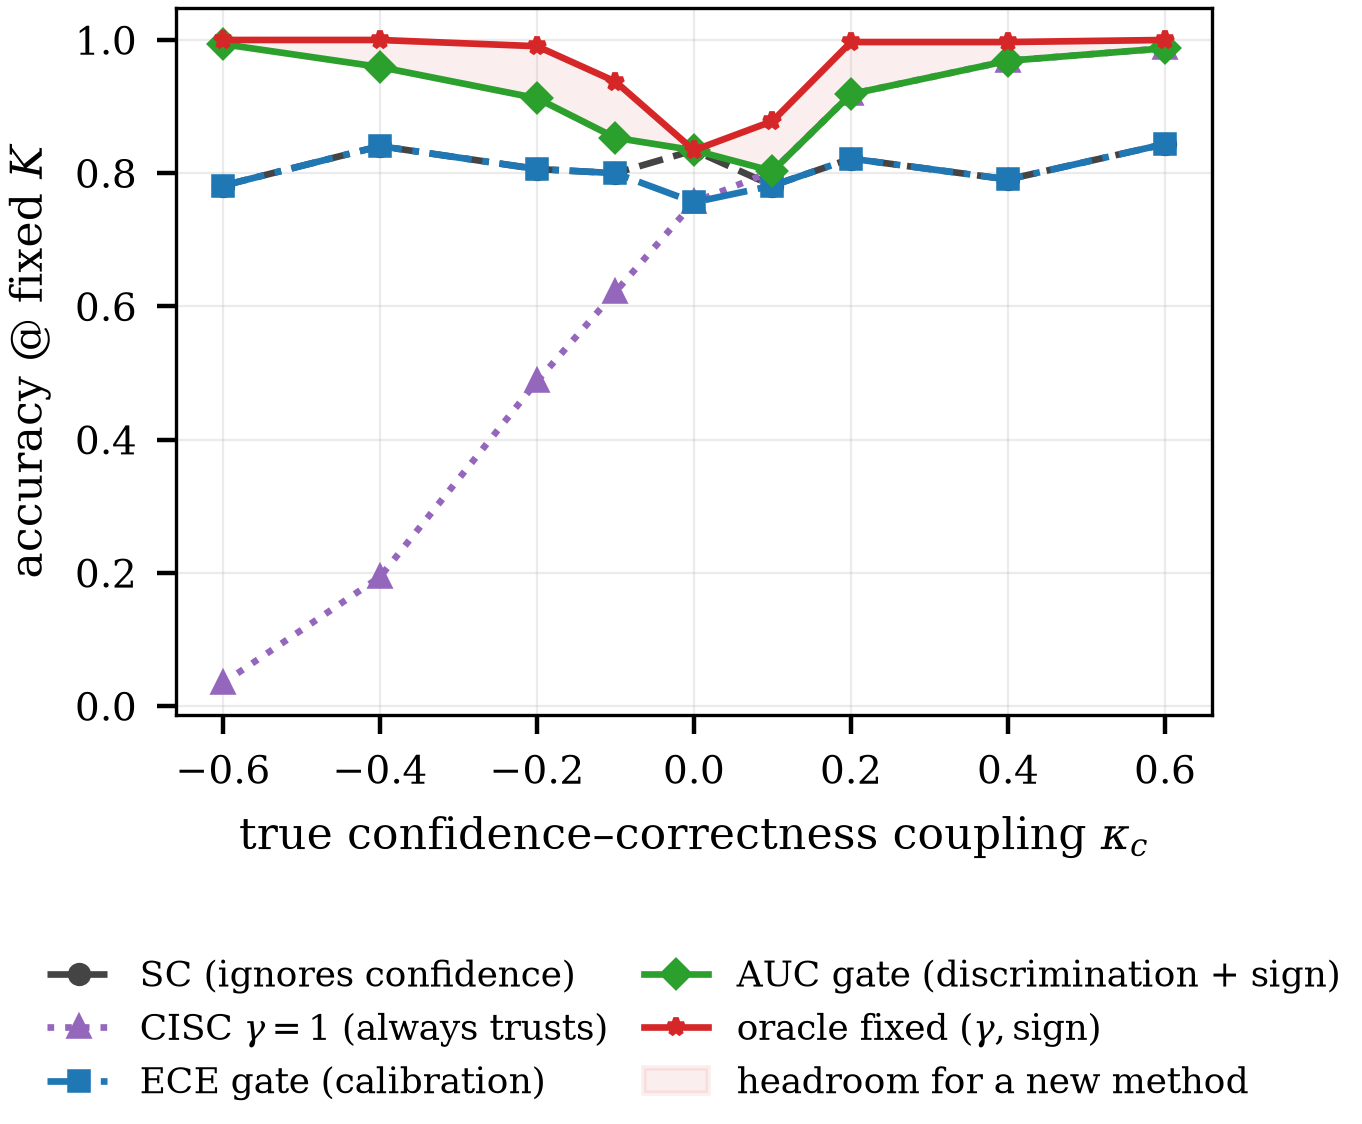
\includegraphics[width=\columnwidth]{figs/kappa_sweep.png}
\caption{The pre-measured problem statement: accuracy of baseline confidence policies at fixed $K{=}15$ as the true coupling $\kappa$ varies. A trivial sign-corrected AUC gate (green) nearly saturates the homogeneous sweep; the headroom for any new method (shaded) concentrates in the mid-range and, off this plot, in distortion, heterogeneity, and label-free cells.}
\label{fig:baselines}
\end{figure}

\section{TACT}\label{sec:method}

\subsection{Vote family}
Within item $q$, let $R_{q,i}$ be the midrank of $c_{q,i}$ (ties averaged) and
\begin{equation}\label{eq:vdw}
\varphi_{q,i}=\frac{v_{q,i}-\bar v_q}{\sigma_q},\qquad v_{q,i}=\Phi^{-1}\!\Big(\frac{R_{q,i}}{m_q+1}\Big),
\end{equation}
where $\sigma_q$ is the \emph{realized} standard deviation of $v$ within the item (the no-tie value is $0.62$ at $m{=}4$ but $0.95$ at $m{=}40$; a closed form would silently rescale $\gamma$ across budgets), and $\varphi\equiv 0$ if $\sigma_q\le 10^{-8}$ (all-tied confidences vote as plain \SC). The vote is
\begin{equation}\label{eq:vote}
\hat a_q=\arg\max_A \sum_{i:\,a_{q,i}=A}\exp\big(\gamma\,\varphi_{q,i}\big),
\end{equation}
and when $\gamma=0$ the implementation \emph{calls the \SC{} routine itself}, making the zero-trust anchor bitwise exact rather than equal in distribution. Because \eqref{eq:vdw} depends on $c$ only through within-item ranks, every strictly monotone distortion of the confidence scale leaves \eqref{eq:vote} unchanged.

\subsection{Reliability statistic}
For item $q$ with $n^1_q$ positive and $n^0_q$ negative labels (dev: $y$; label-free: the pseudo-label of Section~\ref{sec:lf}), the Mann--Whitney statistic on midranks gives
\begin{equation}
D_q = 2\,\mathrm{AUC}_q-1,\qquad \mathrm{AUC}_q=\frac{U_q}{n^1_q n^0_q},
\end{equation}
which equals $2\cdot\mathrm{WQD}_q-1$ in CISC's notation. Pooling uses van Elteren pair-count weights $N_q=n^1_q n^0_q$ \cite{vanelteren1960}:
\begin{equation}\label{eq:pooled}
\Dhat=\frac{\sum_q N_q D_q}{\sum_q N_q}.
\end{equation}
Under the within-item exchangeability null, $U_q$ has the exact tie-corrected variance $n^1_qn^0_q(m_q{+}1)/12\cdot[1-\sum_t(t^3-t)/(m_q^3-m_q)]$, yielding a null standard error $\mathrm{SE}_0$; between-item heterogeneity is captured by the closed-form delete-one-item jackknife $\mathrm{SE}_J$. The conservative choice is
\begin{equation}
\mathrm{SE}=\max\big(\mathrm{SE}_0,\ \mathrm{SE}_J,\ \tfrac{1}{2\sqrt{N}}\big),\qquad r=\Dhat/\mathrm{SE}.
\end{equation}
Because $D$ is a pairwise functional, $\mathbb{E}[\Dhat]$ does not depend on $m_q$: an exponent estimated at $m{=}40$ transfers to deployment at $m{=}8$.

\subsection{Tempering map}
\emph{Shrinkage.} Positive-part James--Stein with a significance floor $\nu$:
\begin{equation}\label{eq:js}
\tilde D=\sign(\Dhat)\,\max\!\big(0,\ |\Dhat|-\nu^2\mathrm{SE}^2/|\Dhat|\big),
\end{equation}
with dead zone $\{|r|\le\nu\}$; $\nu_{\mathrm{dev}}=1.28$, $\nu_{\mathrm{LF}}=2.33$. With $\nu=1$, \eqref{eq:js} is exactly the empirical-Bayes posterior mean under a $\mathcal{N}(0,\tau^2)$ prior with plug-in $\hat\tau^2=\max(0,\Dhat^2-\mathrm{SE}^2)$ \cite{james1961estimation}. The map is odd, continuous, never exceeds $|\Dhat|$, and is monotone in $\Dhat$ and anti-monotone in $\mathrm{SE}$.

\emph{Link.} Model $\varphi\,|\,y\sim\mathcal{N}(\mu_y,s^2)$ within item with the \emph{mixture} standardized to unit variance---which is what \eqref{eq:vdw} enforces---so $s^2=1/(1+\bar p(1-\bar p)u^2)$ where $u=\sqrt2\,\Phi^{-1}\!\big(\tfrac{1+\tilde D}{2}\big)$ and $\bar p$ is the base rate of correct traces. The Bayes-optimal per-trace log-weight coefficient is then
\begin{equation}\label{eq:link}
\gamma^\ast=\frac{u}{s}=u\sqrt{1+\bar p(1-\bar p)\,u^2},
\end{equation}
capped at $\gamma_{\max}$ ($4$ dev, $2$ label-free). The uncorrected link $\gamma=u$ under-weights strong channels by up to ${\sim}50\%$ at $D=0.9$.

\subsection{Anchor properties}
\begin{proposition}[Exact \SC{} reduction]\label{prop:sc}
At $\gamma=0$, \eqref{eq:vote} equals plain \SC{} as a function on every trace pool, including tie-breaks. Under $D=0$, $P(\gamma=0)\to 2\Phi(\nu)-1$ ($80\%$ dev, $98\%$ label-free), and $\gamma$ is continuous through the dead-zone boundary, so a false positive applies an infinitesimal exponent.
\end{proposition}
\begin{proposition}[Exact CISC reduction]\label{prop:cisc}
With the feature map $\varphi^{\log}_{q,i}=\log c_{q,i}-\overline{\log c_q}$, the weights equal $\smash{\kappa_q\,c_{q,i}^{\,\gamma}}$ with a per-item constant $\kappa_q>0$; hence the argmax, the ties, and the normalized vote shares coincide with CISC-power$(\gamma)$ on every pool.
\end{proposition}
\begin{proposition}[Regularity]\label{prop:reg}
The composite $g(\Dhat,\mathrm{SE})$ is continuous, odd, nondecreasing in $\Dhat$, nonincreasing in $\mathrm{SE}$ in magnitude, with $g(D,0^+)=\gamma^\ast(D)$.
\end{proposition}
Proofs are elementary and pinned by unit tests in the released code (76 tests; the permutation-verified null variance, the EB identity in \eqref{eq:js}, and the link derivation \eqref{eq:link} are each tested numerically).

\section{Label-Free Estimation}\label{sec:lf}

\subsection{Pipeline}
(i)~\emph{Dedup:} single-linkage duplicate groups on the lexical-similarity channel at $0.95$; each trace gets weight $1/|\text{group}|$ for plurality determination and pair weighting. (ii)~\emph{Pseudo-label:} $g_{q,i}=\mathbf{1}[a_{q,i}=M_q]$ with $M_q$ the dedup-weighted plurality. (iii)~\emph{Margin gate:} keep the top $60\%$ of items by dedup-weighted margin. (iv)~Compute \eqref{eq:pooled} with $\mathrm{lab}=g$, giving $(\Dhat_g,\mathrm{SE}_g,r_g)$.

\subsection{Sign consistency and its boundary}
\begin{proposition}[Attenuation identity]\label{prop:ccn}
Let $\bar\rho$ be the pair-weighted probability that an item's plurality is wrong. If the plurality-error event is independent of $\varphi$ given $y$ (class-conditional noise), then
$\mathbb{E}[\Dhat_g]=(1-2\bar\rho)\,D$.
In particular $\sign\mathbb{E}[\Dhat_g]=\sign D$ whenever $\bar\rho<1/2$: the label-free estimate can only under-trust, never mis-sign.
\end{proposition}
The identity fails exactly when the flip is \emph{caused} by confidence---a confident echo. There the observable law under $\{$majority right, $D<0\}$ and $\{$majority wrong via confident echo, $D>0\}$ is identical (the two-root ambiguity of \cite{parisi2014ranking} restated for a single channel), so any label-free guarantee is necessarily conditional; it is stated as such rather than papered over.

\subsection{De-attenuation and alarms}
Split-half agreement over $R{=}20$ random half-splits estimates $\alpha=p^2+(1-p)^2/k$ under a one-coin model with $k$ effective wrong alternatives (inverse-Simpson), inverted as $p=[1+\sqrt{1-(k{+}1)(1-k\alpha)}]/(k{+}1)$; $\Dhat_g$ is divided by the \emph{upper} $95\%$ bootstrap bound of $2p-1$ (floored at $0.2$), which can only under-inflate. Four alarms force $\gamma=0$: duplicate collapse (median Kish ratio $<0.5$), sign-aware margin-decoupling, root ambiguity in the split-half quadratic, and insufficient gated items. The margin-decoupling alarm must condition on the estimated trust direction: a sign-naive version (``plurality has the highest mean $\varphi$'') false-alarms on every benign anti-correlated channel---a defect the author hit, diagnosed, and fixed, and which the released tests pin. Finally the significance gate acts on the \emph{raw} $z$ (unbiased sign under Proposition~\ref{prop:ccn}) and temper on the de-attenuated value. A semi-label-free mode takes only the sign from ${\sim}50$ dev labels, routing it into the pipeline and disabling only the proxy-sign alarm; this purchases immunity to the ambiguity above at negligible labeling cost.

\section{Heterogeneity: Impossibility and Escape}\label{sec:hetero}

\subsection{Per-item adaptation is closed under i.i.d.\ coupling}
Suppose $\kappa_q\stackrel{\text{iid}}{\sim}\mathcal{N}(0,0.6^2)$ with no observable covariate.

\begin{proposition}[Self-reinforcement]\label{prop:selfreinf}
Any per-item rule $\gamma_q=h(\Dhat^g_q)$ with $h$ monotone increasing and odd reinforces the plurality on both branches: $\Dhat^g_q>0$ up-weights confident traces, which agree with the plurality; $\Dhat^g_q<0$ up-weights unconfident traces, which are again the plurality side. Empirically such a rule agrees with \SC{} on $97.5\%$ of items and its residual flips are net-harmful ($1$ right vs.\ $9$ wrong per $400$ items).
\end{proposition}

\begin{proposition}[Winner's curse]\label{prop:curse}
On plurality-wrong items with $|D_q|>0.3$---exactly the items where a flip could win---the agreement statistic's sign matches the true sign only $4\%$ of the time.
\end{proposition}

\begin{proposition}[Two-world unidentifiability]\label{prop:twoworld}
For any observed $(a,c)$, the worlds $\{\kappa>0,\ \text{minority correct}\}$ and $\{\kappa<0,\ \text{plurality correct}\}$ induce identical observable laws (constructively, $D$ computed against either truth satisfies $D^{w_1}=-D^{w_2}$). No label-free method can separate them.
\end{proposition}

Consequently the per-item oracle ($0.983$ in this harness) is unreachable, and the honest behaviour is to fall back to the global estimate---which \TACT's dead zone does \emph{exactly}: in the i.i.d.\ cell every variant returns bitwise \SC{} (zero discordant pairs).

\subsection{TACT-group}
Real heterogeneity is typically indexed by an observable covariate (domain, question type). With $\kappa$ indexed by a group label, running the estimator per group keeps every group inside the operating regime of Sections~\ref{sec:method}--\ref{sec:lf}; groups with fewer than $30$ dev (or $60$ unlabeled) items fall back to the global estimate, which Propositions~\ref{prop:selfreinf}--\ref{prop:twoworld} show is the only defensible default.

\section{Experimental Setup}\label{sec:exp}

\textbf{Harness.} A cluster-mixture oracle generates, per item, up to $K_{\max}{=}20$ cached traces with answers, confidences \eqref{eq:confmodel}, and two similarity channels; all methods replay identical pools (paired comparisons, exact McNemar tests). Voting budget $K{=}15$; $400$ items per cell on the sweep, $600$ for the group study; dev splits of $200$ (primary) and $50$ (small-dev).

\textbf{Regimes.} The $\kappa$ sweep $\{-0.6,\dots,+0.6\}$; three strictly monotone confidence distortions (compression toward $0.5$, over-confident sigmoid, fourth power)---rank-preserving by construction, so discrimination is intact while calibration is destroyed; i.i.d.\ heterogeneity ($\kappa_q\sim\mathcal{N}(0,0.6^2)$); covariate-structured heterogeneity (three groups at $+0.6/0/-0.6$); and a confident-echo poison (a wrong cluster echoes verbatim with confidence $0.95$).

\textbf{Baselines.} \SC; CISC-power with $\gamma\in\{0.25,\dots,4\}$; \emph{CISC-devT}, the published dev-calibrated protocol (positive grid picked on dev); a binary ECE gate; \emph{SignGrid-dev}, the strongest trivial baseline (signed exponent grid picked on dev); and the test-set oracle over signed fixed exponents as the upper envelope. The group study adds the naive self-referential per-item method as a negative control and the per-item link oracle as the ceiling.

\textbf{Pre-registered falsifiers.} F1: \TACT-dev significantly below the best fixed-$\gamma$ CISC at $\kappa{=}{+}0.6$. F2: either variant significantly below \SC{} anywhere on the sweep. F3: the label-free variant fails to beat the ECE gate on sweep average. F4: CISC-devT or SignGrid-dev matches \TACT-dev everywhere, including the distortion, heterogeneity, and small-dev cells.

\begin{table}[t]
\centering
\caption{Coupling sweep (accuracy at $K{=}15$; $400$ paired items per cell; dev $n{=}200$). Published protocols sit at the \SC{} floor on the entire negative half-axis.}
\label{tab:sweep}
\setlength{\tabcolsep}{3.4pt}
\begin{tabular}{r cc cc cc c}
\toprule
$\kappa$ & \SC & ECE & devT & SignGrid & \textbf{\TACT-dev} & \textbf{\TACT-LF} & oracle\\
\midrule
$-0.6$ & .807 & .807 & .807 & 1.000 & \textbf{1.000} & \textbf{1.000} & 1.000\\
$-0.4$ & .797 & .797 & .797 & 1.000 & \textbf{1.000} & \textbf{1.000} & 1.000\\
$-0.2$ & .835 & .835 & .835 & .993 & .978 & .978 & .993\\
$-0.1$ & .762 & .762 & .762 & .892 & .880 & .885 & .892\\
$0.0$  & .835 & .835 & .835 & .835 & .835 & .835 & .835\\
$+0.1$ & .795 & .795 & .917 & .917 & .902 & .902 & .917\\
$+0.2$ & .845 & .845 & .993 & .993 & .988 & .988 & .993\\
$+0.4$ & .838 & .838 & 1.000 & 1.000 & \textbf{1.000} & \textbf{1.000} & 1.000\\
$+0.6$ & .782 & .782 & 1.000 & 1.000 & \textbf{1.000} & \textbf{1.000} & 1.000\\
\bottomrule
\end{tabular}
\end{table}

\begin{figure}[t]
\centering
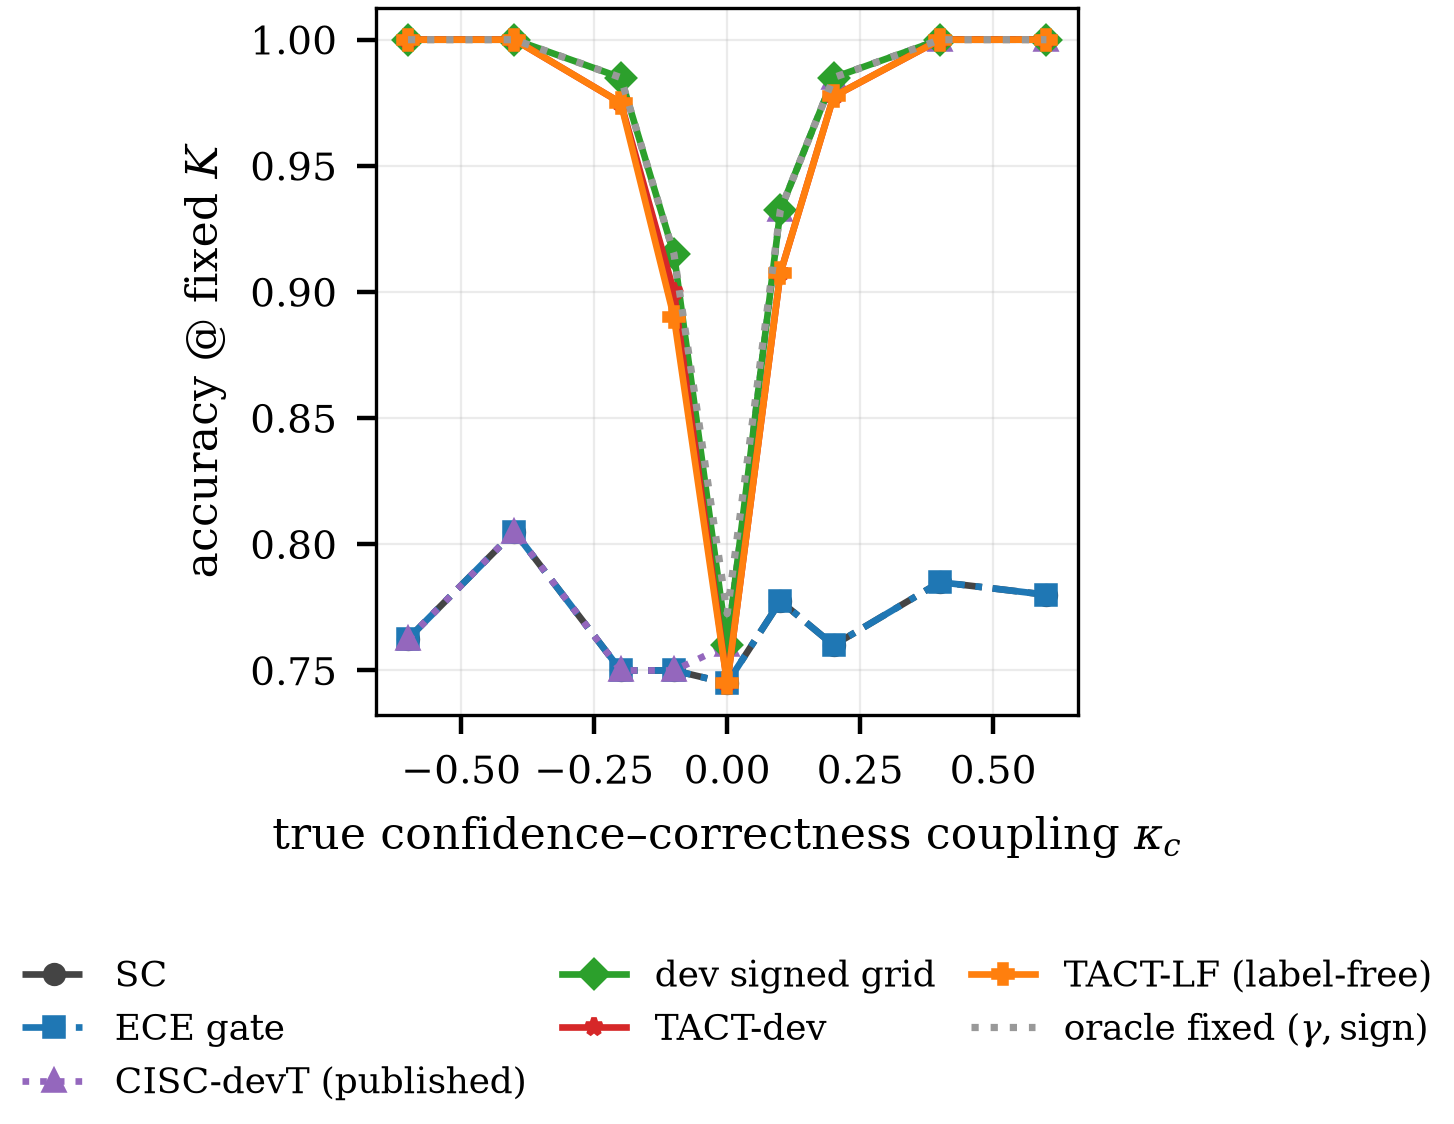
\includegraphics[width=\columnwidth]{figs/tact_sweep.png}
\caption{Main result on the confidence-usage frontier. \TACT-dev and the fully label-free \TACT-LF track the signed oracle across the sweep; CISC-devT and the ECE gate sit at the \SC{} floor for all $\kappa<0$.}
\label{fig:sweep}
\end{figure}

\section{Results}\label{sec:results}

\subsection{Signed recovery, with and without labels}
Table~\ref{tab:sweep} and Fig.~\ref{fig:sweep} give the sweep. Three observations. First, the published protocols never leave the floor on $\kappa<0$: CISC-devT's grid is positive-only and the ECE gate never opens (dev ECE ranges $0.10$--$0.80$ across the sweep while the signal's discrimination is perfect at the extremes). Second, the label-free variant matches the $200$-label variant nearly point-for-point---at $\kappa{=}{-}0.6$ the raw agreement statistic is $\Dhat_g=-0.81$ with $z=-17.6$, and the CCN identity's sign guarantee holds as predicted, yielding $1.000$ with zero labels. Third, at $\kappa=0$ the dead zone returns $\gamma=0$ exactly, so the paired accuracy difference to \SC{} is identically zero---``non-inferior'' is replaced by ``identical.''

\begin{table}[t]
\centering
\caption{Adversarial regimes (accuracy at $K{=}15$). ``Oracle'' is the test-set best over \emph{raw-value} weight policies; rank invariance beats that entire family under compression.}
\label{tab:adv}
\setlength{\tabcolsep}{3.2pt}
\begin{tabular}{l cc cc c}
\toprule
Regime & \SC & devT & SignGrid & \textbf{\TACT-dev} & \textbf{\TACT-LF}\\
\midrule
Monotone compress & .795 & .965 & .965 & \textbf{1.000} & \textbf{1.000}\\
Monotone overconf & .795 & 1.000 & 1.000 & 1.000 & 1.000\\
Monotone power & .795 & 1.000 & 1.000 & 1.000 & 1.000\\
Hetero (i.i.d.) & .810 & .810 & .810 & .810 & .810\\
Confident echo & .200 & .200 & .550 & \textbf{.585} & .200$^{\dagger}$\\
\bottomrule
\multicolumn{6}{l}{\footnotesize $^{\dagger}$alarm fires and the method refuses to leave \SC---the conditional}\\
\multicolumn{6}{l}{\footnotesize guarantee of Prop.~\ref{prop:ccn} working as stated.}
\end{tabular}
\end{table}

\subsection{Rank invariance where raw values fail}
Under monotone compression (Table~\ref{tab:adv}, Fig.~\ref{fig:adv}) all confidences huddle near $0.5$, so every $c^{\gamma}$-family weight is nearly uniform: even the \emph{oracle} over raw-value policies reaches only $0.965$. \TACT's rank scores are untouched by the distortion and both variants reach $1.000$. Under the confident echo, dev labels reveal the inversion (high confidence $\Rightarrow$ wrong) and \TACT-dev counters with $\gamma=-1.20$, the best result in the field ($0.585$; three times the \SC{} floor); label-free, the duplicate-collapse alarm fires and the method correctly refuses---by Proposition~\ref{prop:twoworld} no label-free method could do better than a coin flip on the sign here, and pretending otherwise would be the real failure.

\begin{figure}[t]
\centering

\includegraphics[width=\columnwidth]{figs/tact_adversarial.png}
\caption{Adversarial regimes. Dotted line: the oracle over raw-value weights. Left group of bars: rank invariance beats that family under compression; right: the labeled variant counters the confident echo while the label-free variant alarms and refuses.}
\label{fig:adv}
\end{figure}

\subsection{Heterogeneity}
Table~\ref{tab:group} and Fig.~\ref{fig:group} give the group study. In the covariate-structured cell, per-group \TACT{} recovers each group's signed coupling---dev $\{+4.0,0.0,-4.0\}$, label-free $\{+2.0,0.0,-2.0\}$, the $\kappa{=}0$ group correctly dead-zoned---and cracks the floor that provably binds every global policy: the label-free variant reaches $0.940$, within $0.007$ of the per-item link oracle, with \emph{zero} paired losses to \SC{} over $600$ items ($+79/-0$, $p=3.3\times10^{-24}$). In the i.i.d.\ cell every legitimate method sits at the floor with zero discordant pairs, and the naive self-referential control lands slightly below it---the empirical face of Propositions~\ref{prop:selfreinf}--\ref{prop:twoworld}. One observation is reported as-is rather than tuned for: the label-free variant outperforms the dev variant in the grouped cell ($0.940$ vs.\ $0.923$) because its lower exponent cap ($2$ vs.\ $4$) regularizes better when $|D|\approx1$; cap robustness is left as an ablation.

\begin{table}[t]
\centering
\caption{Heterogeneity study ($600$ paired items; $K{=}15$).}
\label{tab:group}
\setlength{\tabcolsep}{4.5pt}
\begin{tabular}{l cc}
\toprule
Method & Grouped & i.i.d.\\
\midrule
\SC{} (floor) & .808 & .827\\
\TACT{} global (dev) & .808 & .827\\
\TACT-group (dev) & .923 & .827\\
\textbf{\TACT-group (label-free)} & \textbf{.940} & .827\\
Naive per-item (neg.\ control) & .803 & .820\\
Per-item link oracle (ceiling) & .947 & .983\\
\bottomrule
\end{tabular}
\end{table}

\begin{figure}[t]
\centering
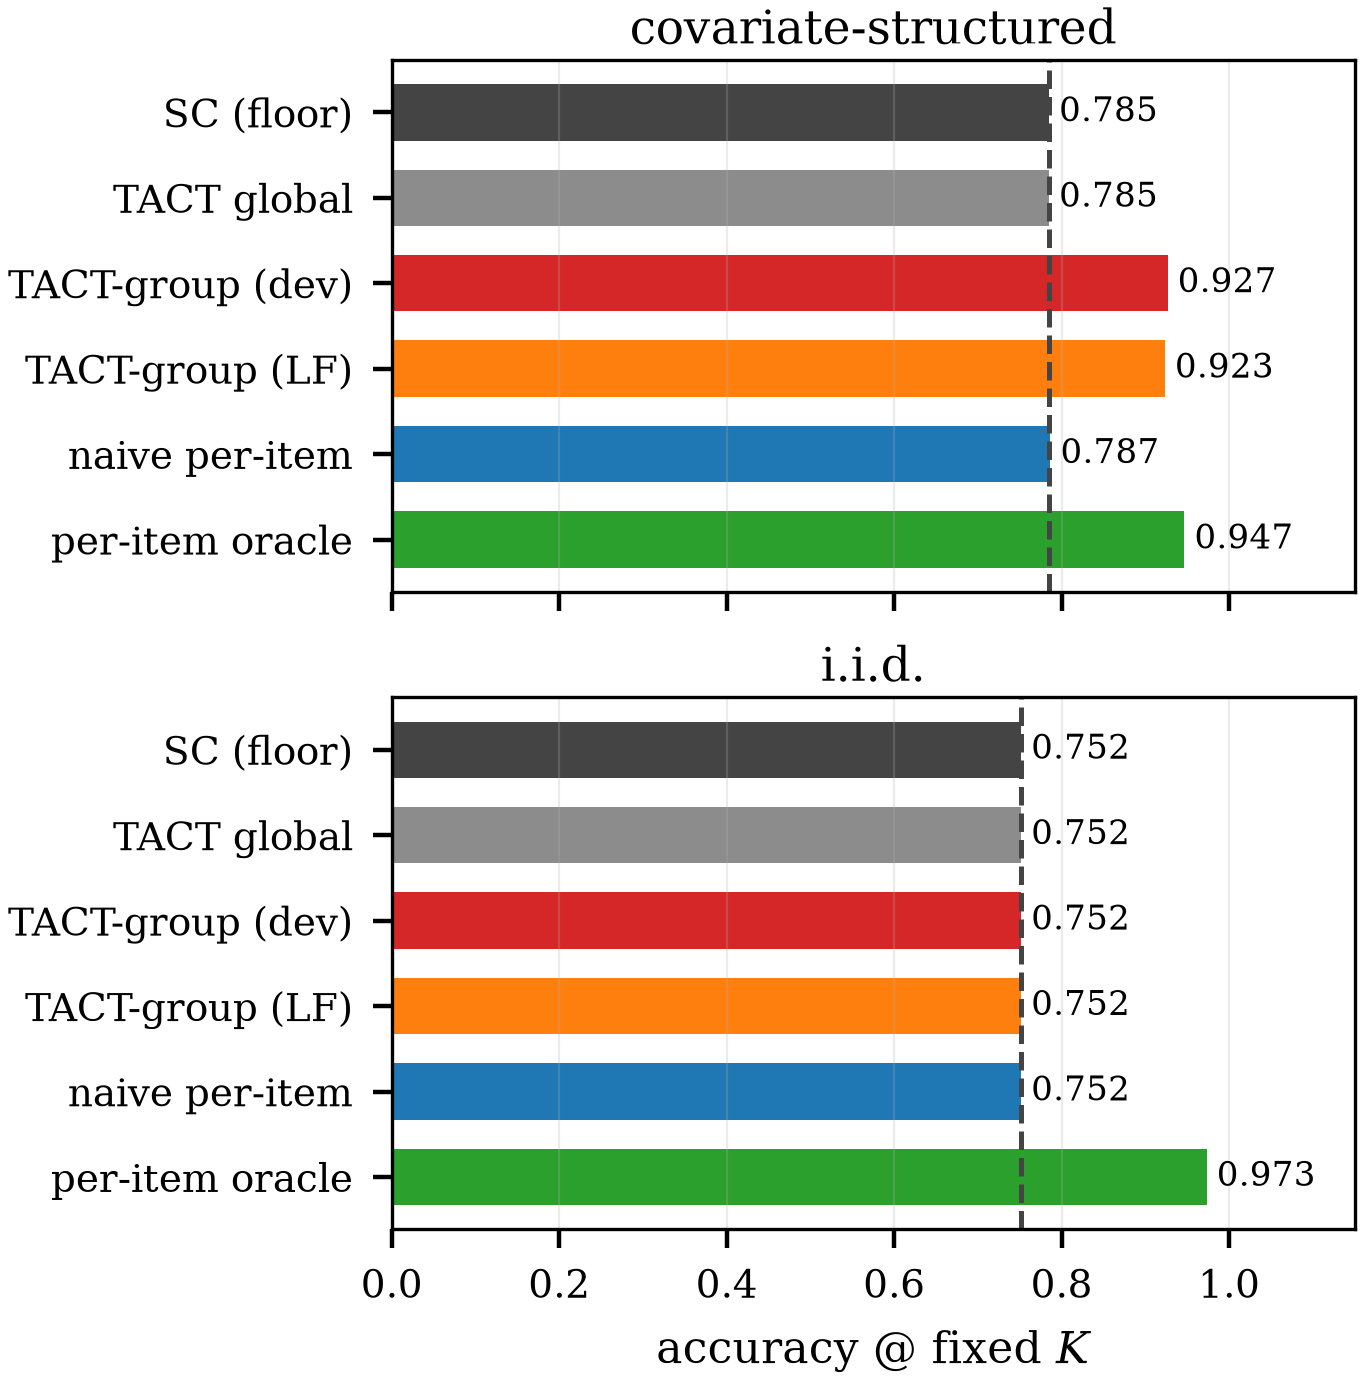
\includegraphics[width=\columnwidth]{figs/group_eval.png}
\caption{Structured vs.\ i.i.d.\ heterogeneity. Left: with an observable covariate, per-group \TACT{} (label-free) approaches the per-item oracle from the $0.808$ floor with zero losses to \SC. Right: the provably closed i.i.d.\ cell---every legitimate method at the floor; the negative control slightly below it.}
\label{fig:group}
\end{figure}

\subsection{Small dev sets and falsifiers}
With dev $n{=}50$ the conclusions are unchanged ($1.000$ at $|\kappa|{=}0.6$; $0.978$ at $-0.2$): the SE-aware shrinkage degrades smoothly rather than catastrophically. All four falsifiers survived: F1 ($1.000$ vs.\ $1.000$), F2 (bit-identical at $\kappa{=}0$; never significantly below \SC{} elsewhere), F3 (sweep means $0.954$ vs.\ $0.811$), and F4 (the distortion and echo cells are unreachable by either grid baseline). Against SignGrid-dev the honest margin is narrow on the homogeneous sweep---\TACT{} even trails by $0.005$--$0.015$ in the mid-range, the deliberate cost of shrinkage---and the net advantage concentrates exactly where pre-registered: distortion ($+0.035$), echo ($+0.035$), and label-free operation, which no grid can perform.

\section{Discussion and Limitations}\label{sec:limits}

\textbf{What the evidence does and does not show.} All quantitative claims are on a synthetic oracle whose confidence model \eqref{eq:confmodel} is, at the homogeneous cells, the very coupling the estimator measures. Three design choices limit the circularity: the adversarial regimes (distortions, heterogeneity, echo) lie outside the estimator's working model; mechanism-recovery claims (does $\Dhat$ track $\kappa$?) are reported separately from accuracy claims; and the pre-measured baseline landscape (Fig.~\ref{fig:baselines}) fixed the winnable cells before the method existed. Validation on real LLM traces is the remaining step; the cached-trace runner is committed and the prediction is falsifiable: if real confidence channels never exhibit directional miscalibration or covariate structure, \TACT's dead zone should make it operationally indistinguishable from CISC-devT there.

\textbf{Narrow margins where labels abound.} When labels are plentiful and the confidence scale is trusted, a dev-picked signed grid captures most of the value; \TACT's case rests on the label-free setting, distorted scales, small dev sets, and the exactness of its anchors.

\textbf{Conditional label-free guarantee.} Proposition~\ref{prop:ccn} requires $\bar\rho<1/2$ after deduplication, and the confident-echo ambiguity is fundamental (Proposition~\ref{prop:twoworld}); the alarms detect the verbatim case only, and paraphrased echo would evade them---the semi-label-free mode is the honest fix at ${\sim}50$ labels.

\textbf{Global exponent per group.} Within a group, \TACT{} ships one exponent; per-item variation inside a group is unexploitable by Propositions~\ref{prop:selfreinf}--\ref{prop:twoworld} unless further covariates exist.

\section{Conclusion}
\TACT{} turns ``how much should this model's confidence be trusted?'' into a measured, signed, uncertainty-aware quantity with exact fallbacks at both ends---plain self-consistency when the evidence is absent, CISC when it is at full strength---and shows that the sign, long unrepresentable in this family of methods, can be recovered without any labels under stated and tested conditions. The accompanying impossibility results draw the boundary that any future per-item method must respect, and the falsification protocol, having already killed one of the author's own systems, is offered as the more portable contribution.

\balance

\begin{thebibliography}{99}\itemsep 1pt

\bibitem{wang2023selfconsistency}
X.~Wang, J.~Wei, D.~Schuurmans, Q.~Le, E.~Chi, S.~Narang, A.~Chowdhery, and D.~Zhou, ``Self-consistency improves chain of thought reasoning in language models,'' in \emph{Proc.\ ICLR}, 2023.

\bibitem{taubenfeld2025cisc}
A.~Taubenfeld \emph{et~al.}, ``Confidence improves self-consistency in LLMs,'' in \emph{Findings of ACL}, 2025, arXiv:2502.06233.

\bibitem{aggarwal2023adaptive}
A.~M. Aggarwal, A.~Madaan, Y.~Yang, and Mausam, ``Let's sample step by step: Adaptive-consistency for efficient reasoning and coding with LLMs,'' in \emph{Proc.\ EMNLP}, 2023.

\bibitem{li2024escape}
Y.~Li \emph{et~al.}, ``Escape sky-high cost: Early-stopping self-consistency for multi-step reasoning,'' in \emph{Proc.\ ICLR}, 2024.

\bibitem{kadavath2022language}
S.~Kadavath \emph{et~al.}, ``Language models (mostly) know what they know,'' arXiv:2207.05221, 2022.

\bibitem{tian2023just}
K.~Tian \emph{et~al.}, ``Just ask for calibration: Strategies for eliciting calibrated confidence scores from language models fine-tuned with human feedback,'' in \emph{Proc.\ EMNLP}, 2023.

\bibitem{xiong2024can}
M.~Xiong \emph{et~al.}, ``Can LLMs express their uncertainty? An empirical evaluation of confidence elicitation in LLMs,'' in \emph{Proc.\ ICLR}, 2024.

\bibitem{huang2024rankcalibration}
X.~Huang \emph{et~al.}, ``Uncertainty in language models: Assessment through rank-calibration,'' arXiv:2404.03163, 2024.

\bibitem{li2023diverse}
Y.~Li \emph{et~al.}, ``Making language models better reasoners with step-aware verifier,'' in \emph{Proc.\ ACL}, 2023.

\bibitem{borda2025}
Z.~Kang \emph{et~al.}, ``Scalable best-of-N selection for large language models via self-certainty,'' arXiv:2502.18581, 2025.

\bibitem{reasc2026}
J.~Kim \emph{et~al.}, ``Reliability-aware adaptive self-consistency,'' arXiv:2601.02970, 2026.

\bibitem{deepconf2025}
Y.~Fu \emph{et~al.}, ``Deep think with confidence,'' arXiv:2508.15260, 2025.

\bibitem{dawid1979maximum}
A.~P. Dawid and A.~M. Skene, ``Maximum likelihood estimation of observer error-rates using the EM algorithm,'' \emph{J.\ Roy.\ Statist.\ Soc.\ C}, vol.~28, no.~1, pp. 20--28, 1979.

\bibitem{whitehill2009whose}
J.~Whitehill \emph{et~al.}, ``Whose vote should count more: Optimal integration of labels from labelers of unknown expertise,'' in \emph{Proc.\ NeurIPS}, 2009.

\bibitem{karger2011iterative}
D.~R. Karger, S.~Oh, and D.~Shah, ``Iterative learning for reliable crowdsourcing systems,'' in \emph{Proc.\ NeurIPS}, 2011.

\bibitem{parisi2014ranking}
F.~Parisi, F.~Strino, B.~Nadler, and Y.~Kluger, ``Ranking and combining multiple predictors without labeled data,'' \emph{Proc.\ Natl.\ Acad.\ Sci.}, vol.~111, no.~4, pp. 1253--1258, 2014.

\bibitem{fuse2026}
Anonymous, ``FUSE: Label-free reliability estimation for ensembles of LLM verifiers,'' arXiv:2604.18547, 2026.

\bibitem{beyondmajority2025}
Anonymous, ``Beyond majority voting: Unsupervised reliability weighting of multiple LLMs,'' arXiv:2510.01499, 2025.

\bibitem{vanelteren1960}
P.~van Elteren, ``On the combination of independent two sample tests of Wilcoxon,'' \emph{Bull.\ Int.\ Statist.\ Inst.}, vol.~37, pp. 351--361, 1960.

\bibitem{james1961estimation}
W.~James and C.~Stein, ``Estimation with quadratic loss,'' in \emph{Proc.\ 4th Berkeley Symp.\ Math.\ Statist.\ Prob.}, 1961, pp. 361--379.

\bibitem{kish1965}
L.~Kish, \emph{Survey Sampling}. New York, NY, USA: Wiley, 1965.

\bibitem{rao1981analysis}
J.~N.~K. Rao and A.~J. Scott, ``The analysis of categorical data from complex sample surveys,'' \emph{J.\ Amer.\ Statist.\ Assoc.}, vol.~76, no.~374, pp. 221--230, 1981.

\bibitem{kuhn2023semantic}
L.~Kuhn, Y.~Gal, and S.~Farquhar, ``Semantic uncertainty: Linguistic invariances for uncertainty estimation in natural language generation,'' in \emph{Proc.\ ICLR}, 2023.

\bibitem{rasc2024}
G.~Wan \emph{et~al.}, ``Reasoning-aware self-consistency: Leveraging reasoning paths for efficient LLM sampling,'' arXiv:2408.17017, 2024.

\end{thebibliography}

\end{document}
